
\section{Constraint matrices}

\subsection{Mass conservation ($C_1$)}

The mass conservation constraint is represented by a matrix where rows
are metabolites, labelled $M = (m_1, \ldots, m_M)$.
Metabolite fluxes must cancel out in order to achive mass conservation.
Note that numerous variables are expressed as concentrations and must be
converted to fluxes as explained previously.

\reffigt{fig:mass_conservation} shows how mass conservation is expressed
in matrix formalism.
The main matrix contains the metabolic reactions,
the production vectors for catalytic elements,
the production/degradation vectors for target elements.
This matrix is growth-rate independent.
The second matrix converts variables that are expressed as
concentrations to fluxes.
This can also be seen as multiplying the appropriate columns in the main matrix
by the growth-rate.

\begin{figure}
  \centering
  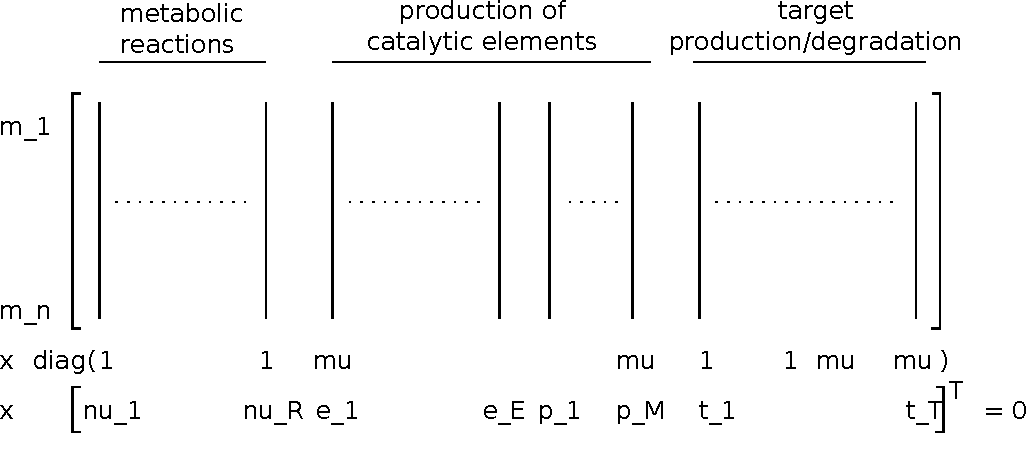
\includegraphics[width=\linewidth]{mass_conservation}
  \caption{Mass conservation constraint.
  Bars in the main matrix are metabolic reaction or
  production/degradation vectors associated with each variable.}
  \label{fig:mass_conservation}
\end{figure}

\subsection{Capacity constraints ($C_2$)}

The capacity constraintes are represented by a matrix where rows are enzymes
or process machineries.
Currently, we use two different formalisms for enzymes and process machineries.

Enzymes are associated to exactly one reaction that may be reversible.
For every enzyme we have the following constraint:
\[
  \nu \leq k_{forward} e_i
\]
where $\nu$ is the flux through the reaction catalyzed by $e_i$.
If the reaction is irreversible, we have the additional constraint
\[
  \nu \geq -k_{backward} e_i
\]
In order to write all constraints, we need a reaction to enzyme mapping.
This is represented by a matrix where we have one row per constraint.
Each row has a 1 on the column corresponding to the reaction catalyzed,
and 0s everywhere else.

Process machineries participate in the synthesis/degradation of several
macromolecules (enzymes, machineries and targets).
For every target, we have a constraint of the form
\[
   [machinery\_cost].[E, P, T]^T \leq k_{machinery} p_i
\]
Every macromolecule has a set of machinery costs associated with it.
It tells how much a machinery is used in order to produce/degrade the
macromolecule (the cost is often 0).

The final matrices are very sparse \reffigp{fig:capacity_constraints}.
A first matrix contains the reaction to enzyme mapping and the machinery
costs. This matrix is growth-rate independent.
A second matrix contains efficiencies, that may depend on growth-rate.
Note that we did not need to convert concentrations to fluxes here.

\begin{figure}
  \centering
  \includegraphics[width=\linewidth]{capacity_constraints}
  \caption{Capacity constraints.}
  \label{fig:capacity_constraints}
\end{figure}

\subsection{Density constraints ($C_3$)}

Density constraints are represented by matrices where rows are compartments,
labelled $C = (c_1, \ldots, c_C)$.

Every variable that represents a concentration participates to this constraint.
For every macromolecule, we define a weight vector that defines how much
volume one molecule occupies in every compartment (in user defined units).
By putting these vectors together we get a weight matrix.

The user also defines a vector of maximal weights for every compartment,
yielding a simple set of constraints \reffigp{fig:density_constraints}.
Only the right-hand part may contain growth-rate dependent values.
Again, no conversion from concentration to flux is needed here.

\begin{figure}
  \centering
  \includegraphics[width=\linewidth]{density_constraints}
  \caption{Density constraints.}
  \label{fig:density_constraints}
\end{figure}
